\documentclass{seal_thesis}

\usepackage[
  top=1.25in,
  bottom=1.25in,
  left=1.25in,
  right=1.25in
]{geometry}

\thesisType{Master Project Report}
\date{\today}
\title{GLAPP}
\subtitle{}
\author{
Fabio Isler \textmd{(09-115-965)} \\
Adrian Li \textmd{(XX-XXX-XXX)} \\
Dinesh Pothineni \textmd{(XX-XXX-XXX)} \\
Riccardo Patane \textmd{(XX-XXX-XXX)}}
\home{} % Geburtsort
\country{}
\prof{Prof. Dr. Harald C. Gall}
\assistent{Dr. Philipp Leitner}
\email{}

\begin{document}
\maketitle

\abstract
Abstract


%%%%%%%%%%%%%%%%%%%%%%%%%%%%%%%%%%%%%%%%%%%%%%%%%%%%%%%%%
% NEW CHAPTER																						%
% Remember to always use a new line for a new sentence! %
%%%%%%%%%%%%%%%%%%%%%%%%%%%%%%%%%%%%%%%%%%%%%%%%%%%%%%%%%
\chapter{Introduction}
Cloud computing has created a paradigm shift in the last few years, by making infrastructure available at lower costs and with higher efficiency of operations.
These solutions are increasingly being adopted by enterprises and developers, as they can provision huge amount of resources to scale on-demand in order to meet their business needs.
In cloud computing, resources such as CPU processing time, disk space, or networking capabilities, are rented and released as a service.
Today, the most important model for delivering on the cloud promise is the Infrastructure-as-a-Service (IaaS) paradigm.
In IaaS, virtual computing resources are acquired and released on demand, either via an Application Programming Interface (API) or web interface.
Along with great flexibility of being able to get new resources on demand and pay for what you use, new problems arise.
Selecting a cloud service provider can often be a quite challenging decision for the developer or a company, so is being able to monitor and evaluate these infrastructure resources on a regular basis.
With so much of variance in cost and performance, it is imperative that one would look for a reliable deployment, monitoring solutions to strike a balance with application requirements.
Furthermore, the complexity and skill required to manage multiple layers of application, data, middleware and operating systems can .

Understanding run time performance, behavior of various application components in realtime can enable us to take advantage of arbitrage opportunities that exist between different machines/regions or even other cloud providers.
For example, an application can take advantage by moving closer to its users based on timezones or traffic to improve response time.
Currently there is no flexibility to move freely between various cloud providers without great development effort and cost, however such an ability to move freely between providers enables us to benefit from cost and performance differences.
We propose a cloud middleware that can take not only take care of application deployment to cloud, but also constantly monitor and trigger such necessary adaptations to benefit from these opportunities.
Ideally this middleware also enables developers to specify their intended goals in terms of high level policies to govern the application behavior.
The middleware can then break down these policies into low level objectives, in order to trigger adaptations by changing the state of application when required.

%%%%%%%%%%%%%%%%%%%%%%%%%%%%%%%%%%%%%%%%%%%%%%%%%%%%%%%%%
% NEW SECTION																						%
%%%%%%%%%%%%%%%%%%%%%%%%%%%%%%%%%%%%%%%%%%%%%%%%%%%%%%%%%
\section{Global Living Cloud Applications}

The aim of this project is to develop a middleware for what we call ''global living cloud applications'' (GLAs).
In a nutshell, GLAs are a bio-inspired notion of cloud-native applications.
GLAs ''live'' in the cloud, and are able to migrate between data centers and cloud providers automatically, based on changes in cost and performance of cloud offerings, changes in customer behavior or requirements, or other factors.

\todo{''What I would really do is invest more thought and discussions on the conceptual model behind GLAs - I think there is something pretty cool here, but it does not seem very well-developed to me.''}


The bio-inspired terminology applies for the different levels of components of a GLA:

\begin{itemize}
	\item Cell: A cell is the lowest-level component of a GLA, consisting of the actual processes \todo{''I wonder whether it makes sense to equate cells to "processes". Is that really the same?''}
	\item Organ: An organ consists of one or more cells of the same type \todo{''For organs, I understand that organs typically also have cells of different type, i.e., an injected load balancer. I would try to make the model clear in this regard. For instance, it may make sense to distinguish between cells that are user-defined and those that come from your middleware.''}
	\item GLA: The GLA itself is a collection of organs that form the whole application
\end{itemize}

In order to manage these GLAs, we introduce a middleware called GLAPP (Global Living Application Platform).
It allows a developer to deploy multiple GLAs on whatever cloud he/she has access to and sets a centralized mechanism in place to constantly monitor and manage all the GLAs.
The middleware supports heterogeneous environment a GLA can live and move across different providers, regions, instance types, etc.
GLAPP is an open source middleware to be used on a private/individual basis.
This means that in order to be able to deploy a GLA through GLAPP, it is first required to install the GLAPP platform on the own infrastructure.
But no matter where the platform is installed, all GLAs will live in the cloud.


%%%%%%%%%%%%%%%%%%%%%%%%%%%%%%%%%%%%%%%%%%%%%%%%%%%%%%%%%
% NEW SECTION																						%
%%%%%%%%%%%%%%%%%%%%%%%%%%%%%%%%%%%%%%%%%%%%%%%%%%%%%%%%%
\section{GLAPP Architecture}
The middleware consists of 3 different parts/blocks: a front end, a provisioning component and a control loop.
The front end provides an interface for developer to interact with the middleware to deploy and manage his/her GLAs.
The provisioning component provides the management functionalities of the middleware including cloud infrastructure management, application deployment and access to the application status information.
Lastly the control loop is the component responsible for enabling the management of GLAs by the middleware itself.
It follows the MAPE (Monitoring, Analysis, Planning and Execution) principle.
Possible execution actions are moving cells between different cloud instances (migration), duplicating/splitting cells of the GLA (mitosis), or removing cells.

\begin{figure}[!ht]
\centering
	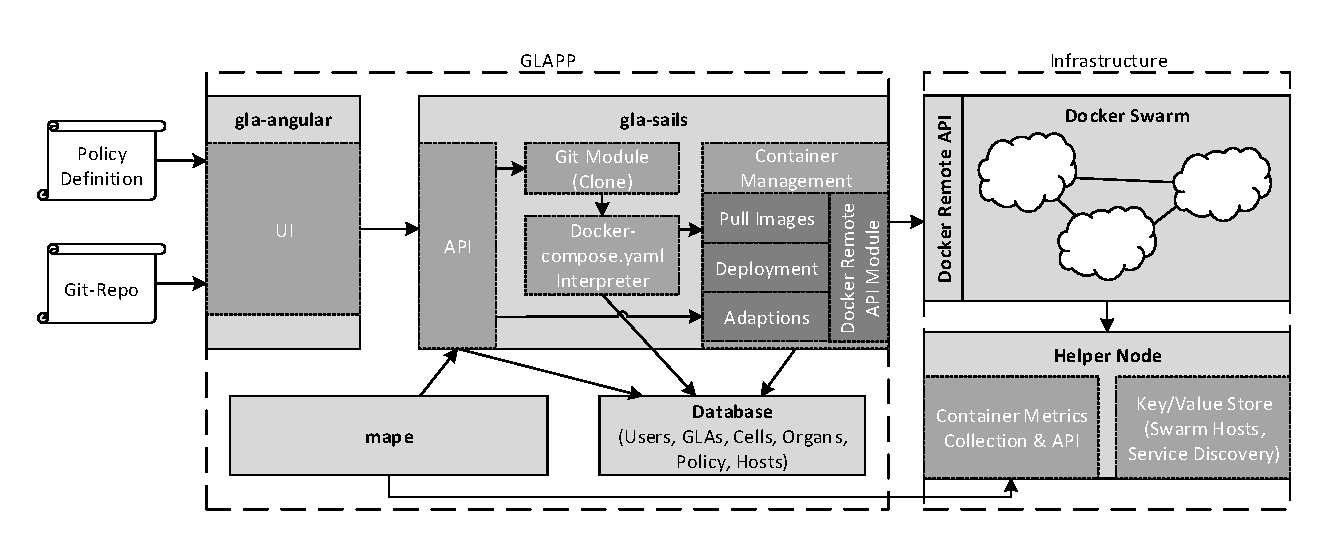
\includegraphics[width=\textwidth]{detailed_architecture.pdf}
	\caption{Detailed Architecture of GLAPP and the Infrastructure}
	\label{fig:detailed}
\end{figure}
\todo{Explain the not yet mentioned parts - maybe, this detailed architecture is rather part of the ''Current State'' chapter, then we need to include a basic architecture here}

\noindent\todo{''I like Fig2 better, but there is still plenty of room for improvement. For instance, I would remove the word "optimal" from the figure - especially, if we now use this iterative Q-learning approach, our deployment will often *not* be optimal, at least temporarily. I am also quite suspicious that the msot dominant block in the figure is the provisioner. Is this really what we want to emphasize?''}


%%%%%%%%%%%%%%%%%%%%%%%%%%%%%%%%%%%%%%%%%%%%%%%%%%%%%%%%%
% NEW CHAPTER																						%
% Remember to always use a new line for a new sentence! %
%%%%%%%%%%%%%%%%%%%%%%%%%%%%%%%%%%%%%%%%%%%%%%%%%%%%%%%%%
\chapter{Work}


%%%%%%%%%%%%%%%%%%%%%%%%%%%%%%%%%%%%%%%%%%%%%%%%%%%%%%%%%
% NEW SECTION																						%
%%%%%%%%%%%%%%%%%%%%%%%%%%%%%%%%%%%%%%%%%%%%%%%%%%%%%%%%%
\section{Basic Design Decisions}

\subsection{Main Components: Provisioning Backend, Frontend, MAPE}
\todo{Describe the design decisions of the main components}

\subsection{Deployment: Containerization with Docker}
\subsubsection{Containerization vs. other virtualization methods:}
\todo{Explain the advantage of containerization compared to e.g. virtual machines}
\subsubsection{Docker vs. other containerization implementations:}
\todo{Explain the advantage of Docker compared to e.g. OpenVZ}

\subsection{Orchestration: Docker Swarm}
\todo{Explain the advantage of Docker Swarm compared to e.g. Kubernetes}


%%%%%%%%%%%%%%%%%%%%%%%%%%%%%%%%%%%%%%%%%%%%%%%%%%%%%%%%%
% NEW SECTION																						%
%%%%%%%%%%%%%%%%%%%%%%%%%%%%%%%%%%%%%%%%%%%%%%%%%%%%%%%%%
\section{Implementation Decisions}
\subsection{Backend: Node.js}
\todo{Explain the choice and alternatives}

\subsection{GUI: AngularJS}
\todo{Explain the choice and alternatives}

\subsection{MAPE: Java}
\todo{Explain the choice and alternatives}


%%%%%%%%%%%%%%%%%%%%%%%%%%%%%%%%%%%%%%%%%%%%%%%%%%%%%%%%%
% NEW CHAPTER																						%
% Remember to always use a new line for a new sentence! %
%%%%%%%%%%%%%%%%%%%%%%%%%%%%%%%%%%%%%%%%%%%%%%%%%%%%%%%%%
\chapter{Current State}



%%%%%%%%%%%%%%%%%%%%%%%%%%%%%%%%%%%%%%%%%%%%%%%%%%%%%%%%%
% NEW CHAPTER																						%
% Remember to always use a new line for a new sentence! %
%%%%%%%%%%%%%%%%%%%%%%%%%%%%%%%%%%%%%%%%%%%%%%%%%%%%%%%%%
\chapter{Case Study}



%%%%%%%%%%%%%%%%%%%%%%%%%%%%%%%%%%%%%%%%%%%%%%%%%%%%%%%%%
% NEW CHAPTER																						%
% Remember to always use a new line for a new sentence! %
%%%%%%%%%%%%%%%%%%%%%%%%%%%%%%%%%%%%%%%%%%%%%%%%%%%%%%%%%
\chapter{Conclusion}


\bibliographystyle{alpha}
\bibliography{sources}

\end{document}
